\section{Schaltvorgänge}
\subsection{Berechnungsmethoden}
Immer \textbf{Stetigkeitsbedingungen} beachten!
\[
\boxed{x(t=0) = x(0) = x(0^-) = x(0^+)}
 \]
Bauteilverhalten KS/LL:
 $\underline{X}_C=-j\frac{1}{\omega C}$ \quad $\underline{X}_L =j \omega L$
\subsubsection{Vereinfachte Methode}
mit Lösungsformeln aus GE1, GE2.
\begin{itemize}
	\item \textbf{Bedingung}: \textbf{konstantes} Eingangssignal/Quelle und \textbf{einem} unabhängigem Energiespeicher $L$ \textbf{oder} $C$ (DGL 1. Ordnung, \textbf{eine} Zeitkonstante).
	\item GE1: Schaltung mit \textbf{einer} Induktivität $L$:
	\begin{gather*}
		\tau=\frac{L}{R} \qquad I_A = i(0) \qquad I_E=i(t\rightarrow\infty)\\
		\boxed{i(t)=I_E+(I_A-I_E)\cdot e^{-t/\tau}}
	\end{gather*}
	\item GE2: Schaltung mit \textbf{einer} Kapazität $C$:
	\begin{gather*}
		\tau=RC \qquad U_A = u(0) \qquad U_E=u(t\rightarrow\infty)\\
		\boxed{u(t)=U_E+(U_A-U_E)\cdot e^{-t/\tau}}
	\end{gather*}
	
\end{itemize}

\subsubsection{Laplace-Transformation der DGL}\label{lpt_dgl_ableitung}
\begin{enumerate}
	\item DGL aufstellen mit Bauteilgleichungen f\"ur $R,L,C$. Maschen- und Knotensatz anwenden.
	\item LPT der DGL durchführen:
\begin{align*}
	\dot{x}(t) \ &\laplace\ s\cdot\underline{X}(s)-x(0)\\
	\ddot{x}(t) \ &\laplace\ s^2\cdot\underline{X}(s)-s\cdot x(0)-\frac{dx}{dt}(0)\\
	x^{(3)}(t) \ &\laplace\ s^3\cdot\underline{X}(s)-s^2\cdot x(0)-s\cdot \frac{d}{dt}x(0) - \frac{d^2}{dt}x(0)
\end{align*}
	Anfangszustand $i_L, u_C \neq 0$ zum Schaltzeitpunkt $x(0)$ wird autom. \textbf{berücksichtigt}.
	\item Auflösen nach gesuchter Größe.
	\item Rücktransformation in Zeitbereich mit \textbf{Tabelle}.
\end{enumerate}

\subsubsection{Leere Energiespeicher mit LPT \& KWR}
\begin{enumerate}
	\item \textbf{Bedingung}: Alle $C$ ungeladen, Alle $L$ stromlos.
	\[ 
	 u_c(0+) = i_L(0+) = 0
	 \]

	\item Eingang $x(t)$ mit LPT in Bildbereich $\underline{X}(\omega)$.
    \item $\underline{H}(s)$ aus Schaltung \underline{nach}
        Schaltvorgang mit erweiteter KWR bestimmen. Ersetze $s = j\omega $.
    \item Ausgang im Bildbereich berechnen: $\underline{Y}(s) =
        \underline{X}(s)\cdot \underline{H}(s)$
    \item Rücktransformation in Zeitbereich mit \textbf{Tabelle}.
    
\end{enumerate}
\subsubsection{Geladene Energiespeicher mit LPT}
\begin{enumerate}
    \item Ersatzschaltbild (ESB) für Schaltkreis nach dem
        Schaltvorgang im Bildbereich erstellen:
        \begin{itemize}
        	\item VZ beachten! VZ-Änderung im Zeitbereich auch im Bildbereich gültig!
            \item Induktivitäten mit Anfangsstrom:
            
                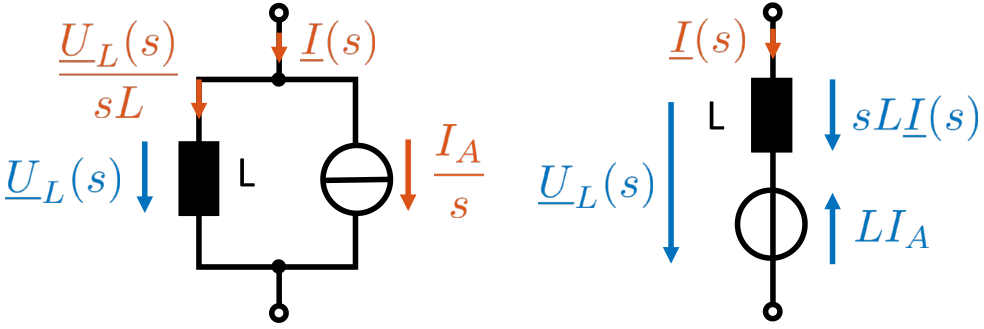
\includegraphics[width=0.4\textwidth]{Bilder/ESB_Fuer_stromfuehrende_Induktivitaet}
                
                \begin{align*}
                    \underline{U}_L(s) &= L\cdot(s\cdot\underline{I}_L(s)-\underbrace{i_L(0)}_{I_A})\\
                    \underline{I}_L(s) &= \frac{\underline{U}_L(s)}{sL}+\frac{I_A}{s}
                \end{align*}
            \item Kapazitäten mit Anfangsspannung/Vorladung:
                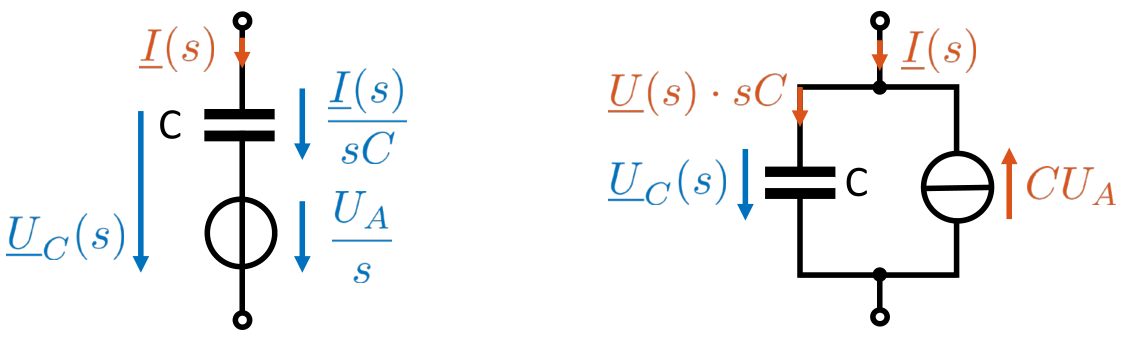
\includegraphics[width=0.4\textwidth]{Bilder/ESB_Fuer_geladene_Kapazitaet}
                \begin{align*}
                    \underline{I}_C(s) &= C\cdot(s\cdot\underline{U}_C(s)-\underbrace{u_C(0)}_{U_A})\\
                    \underline{U}_C(s) &= \frac{\underline{I}_C(s)}{sC}+\frac{U_A}{s}
                \end{align*}
        \end{itemize}
    \item $\underline{H}(s)$ aus ESB mit KWR bestimmen.
    \item Eingang $x(t)$ mit LPT in Bildbereich $\underline{X}(\omega)$.
    \item Ausgang im Bildbereich berechnen: $\underline{Y}(s) =
        \underline{X}(s)\cdot \underline{H}(s)$
    \item Rücktransformation in Zeitbereich mit \textbf{Tabelle}.
\end{enumerate}
\subsection{Quellenumwandlung}
\begin{gather*}
	\text{Stromquelle: }i_q(t)\cdot \varepsilon(t) \quad \laplace \quad \frac{I_q(s)}{s}\\
	\text{Spannungsquelle: }u_q(t)\cdot \varepsilon(t) \quad \laplace \quad \frac{U_q(s)}{s}
\end{gather*}
\subsection{Bauteilgleichungen}
\begin{gather*}
	i_L (t) = C \cdot \frac{du_c(t)}{dt} \qquad u_L (t) = L \cdot \frac{di_c(t)}{dt}
\end{gather*}